\documentclass[12pt]{exam}
\usepackage{amsthm}
\usepackage{bm}
\usepackage{libertine}
\usepackage[utf8]{inputenc}
\usepackage[margin=0.5in]{geometry}
\usepackage{amsmath,amssymb}
\usepackage{multicol}
\usepackage[shortlabels]{enumitem}
\usepackage{siunitx}
\usepackage{physics}
\usepackage{booktabs}
\usepackage{graphicx}
\usepackage{pgfplots}
\usepackage{listings}
\usepackage{tikz}

\bmdefine{\ii}{i}                       %% cuaternion i
\bmdefine{\jj}{j}                       %% cuaternion j
\bmdefine{\kk}{k}                       %% cuaternion k
\newcommand{\te}{\theta}                %% short for  \theta

\newcommand{\word}[1]{\quad\text{#1}\quad} %% texto intercalado


\pgfplotsset{width=10cm,compat=1.9}
\usepgfplotslibrary{external}
\tikzexternalize

\newcommand{\class}{Math 261-001} % This is the name of the course 
\newcommand{\examnum}{Quiz 5} % This is the name of the assignment
\newcommand{\examdate}{October 3} % This is the due date





\begin{document}
\pagestyle{plain}
\thispagestyle{empty}

\noindent
\textbf{\class}\\
\textbf{\examnum}, \textbf{\examdate} \\

% Name \hfill CSU ID \# \hspace{2.25in}

%\vspace{10 pt}

\setlength{\tabcolsep}{3.5cm} % Default value: 6pt
\renewcommand{\arraystretch}{1.5}
\setlength\extrarowheight{1cm}
\begin{tabular}{ |c|c| } 
 \hline
 Name   & CSU ID \#  \\ 
 \hline
\end{tabular}
% ---
\vspace{10pt}
\iffalse

    \foreach \s in {1,...,5}{
          \choice $P_\s$ has no power 
     }%;
\fi

Be sure to read each question carefully. You must choose and answer \textbf{exactly two} of the four problems.  
If you attempt more than two, only the first two will be graded.  
Write your final answers in the boxes provided. Each problem is worth the same amount of points.  
\textbf{Each problem is accompanied by a figure to help you visualize the region of integration.}  


\begin{enumerate} 

\item Consider the integral 
$$\int_{-2}^0\int_{\sqrt{4-x^2}}^{\sqrt{16-x^2}}f(x,y)\,dy\,dx.$$
By changing to polar coordinates, rewrite this integral as the sum of two integrals in polar form.
\begin{flushleft}
    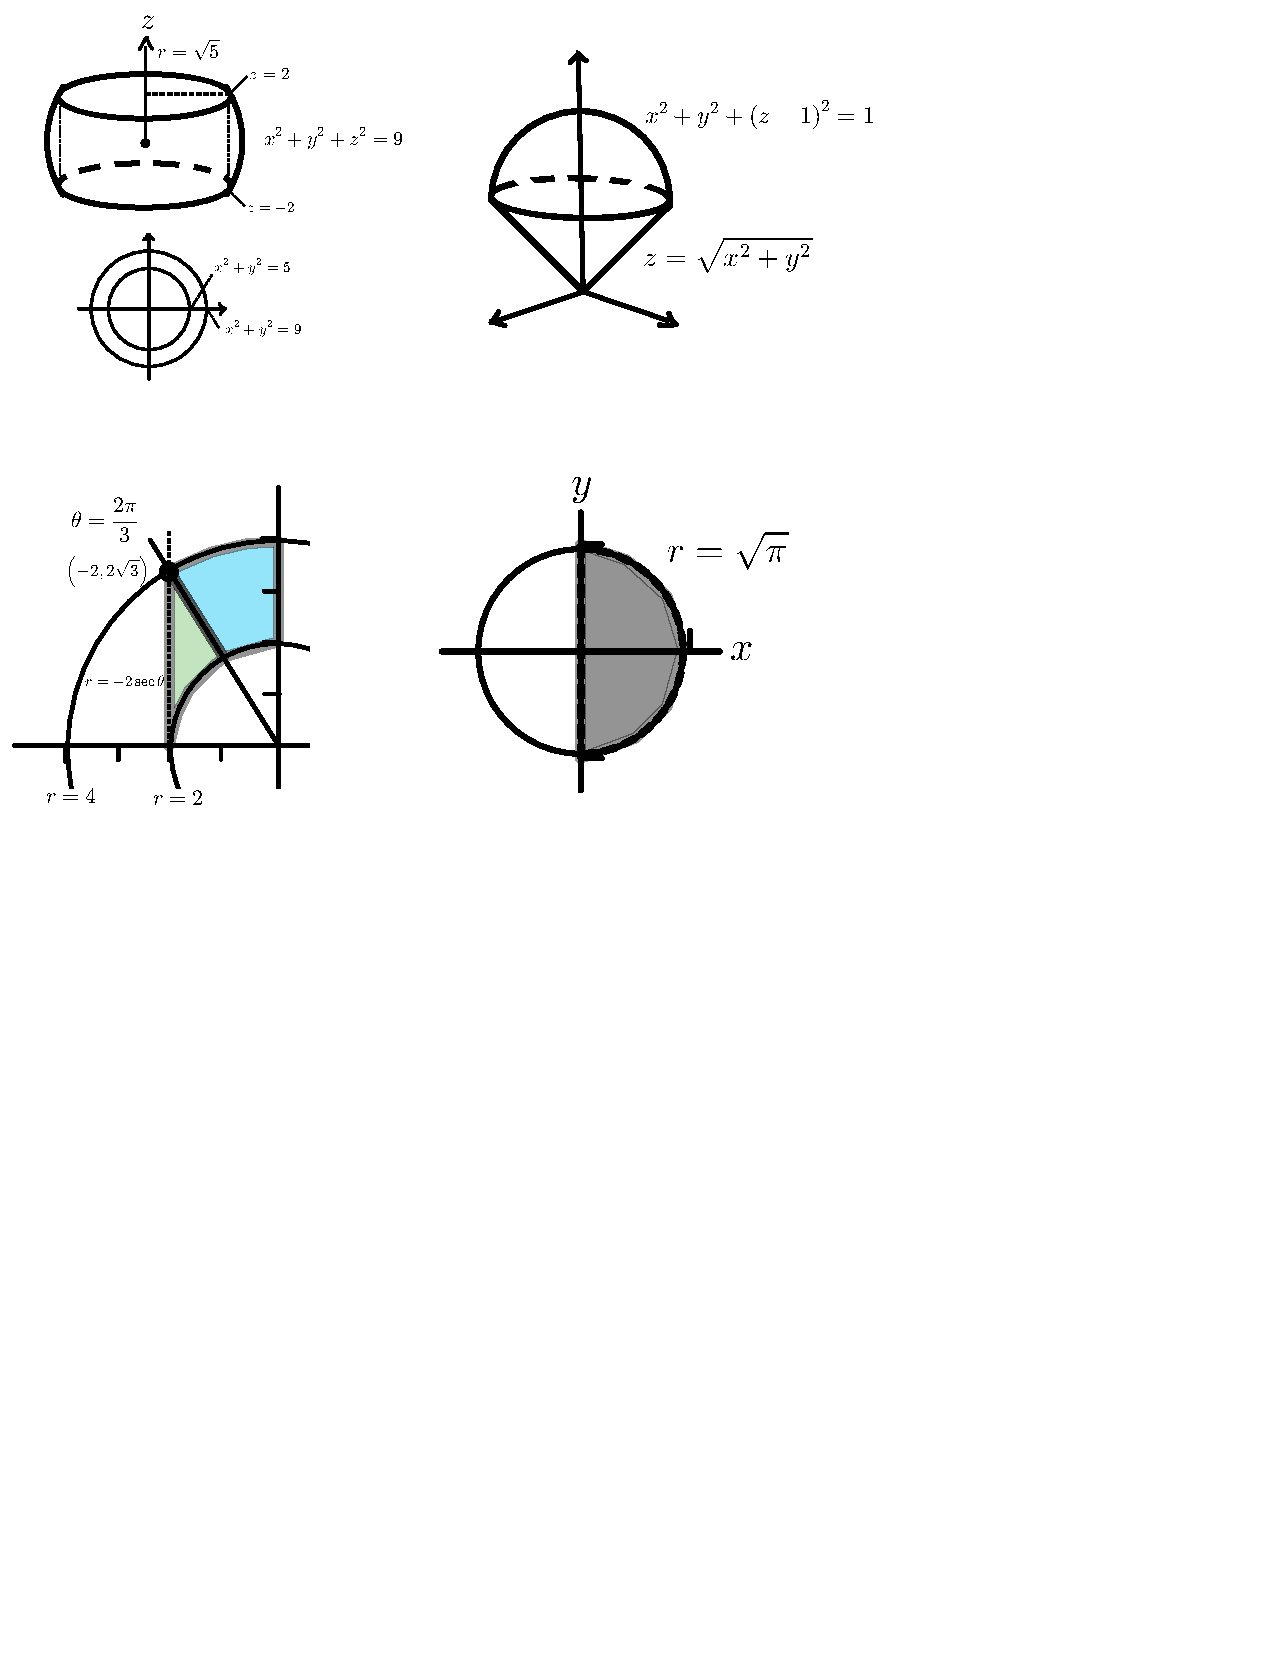
\includegraphics[width=0.3\textwidth, trim=0.5cm 14.5cm 16.5cm 8cm,clip]{figs.pdf}\hfill 
\framebox(320,50){}
\end{flushleft}

\item Evaluate the double integral 
$$\int_{-\sqrt{\pi}}^{\sqrt{\pi}}\int_{0}^{\sqrt{\pi-y^2}}\sin(x^2+y^2)\,dx\,dy$$
by changing to polar coordinates, and \textbf{compute its exact value}.
\begin{flushleft}
    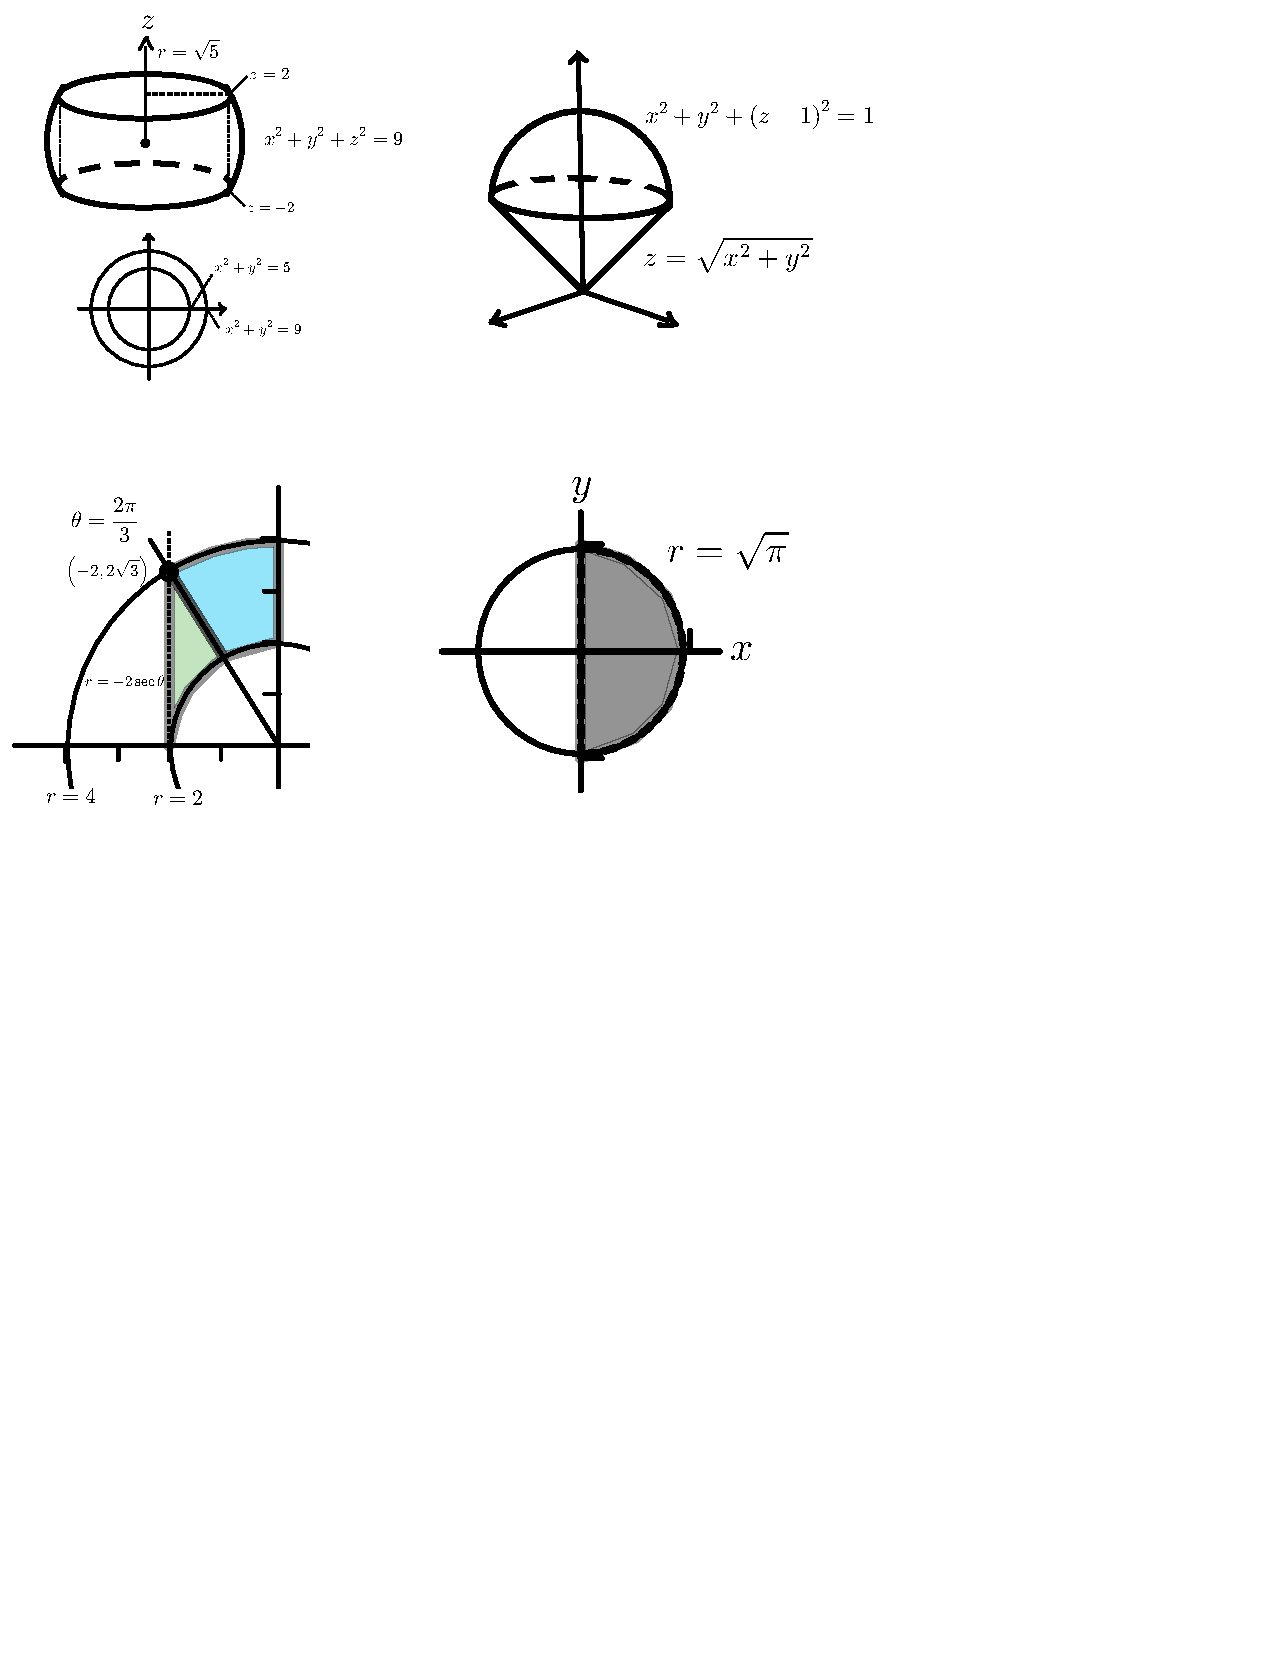
\includegraphics[width=0.3\textwidth, trim=7.5cm 15cm 8cm 8cm,clip]{figs.pdf}\hfill 
\framebox(320,50){}
\end{flushleft}

\newpage

\item You're walking in your favorite supermarket and spot a \textbf{cheese wedge}! You decide to calculate its volume using cylindrical coordinates.  
Model the wedge as the region bounded by
$$x^2+y^2+z^2=9, \quad z=2, \quad z=-2.$$
Using the cylindrical substitution $x=r\cos\theta,\ y=r\sin\theta,\ z=z$, set up an integral expression for the volume.
\begin{flushleft}
    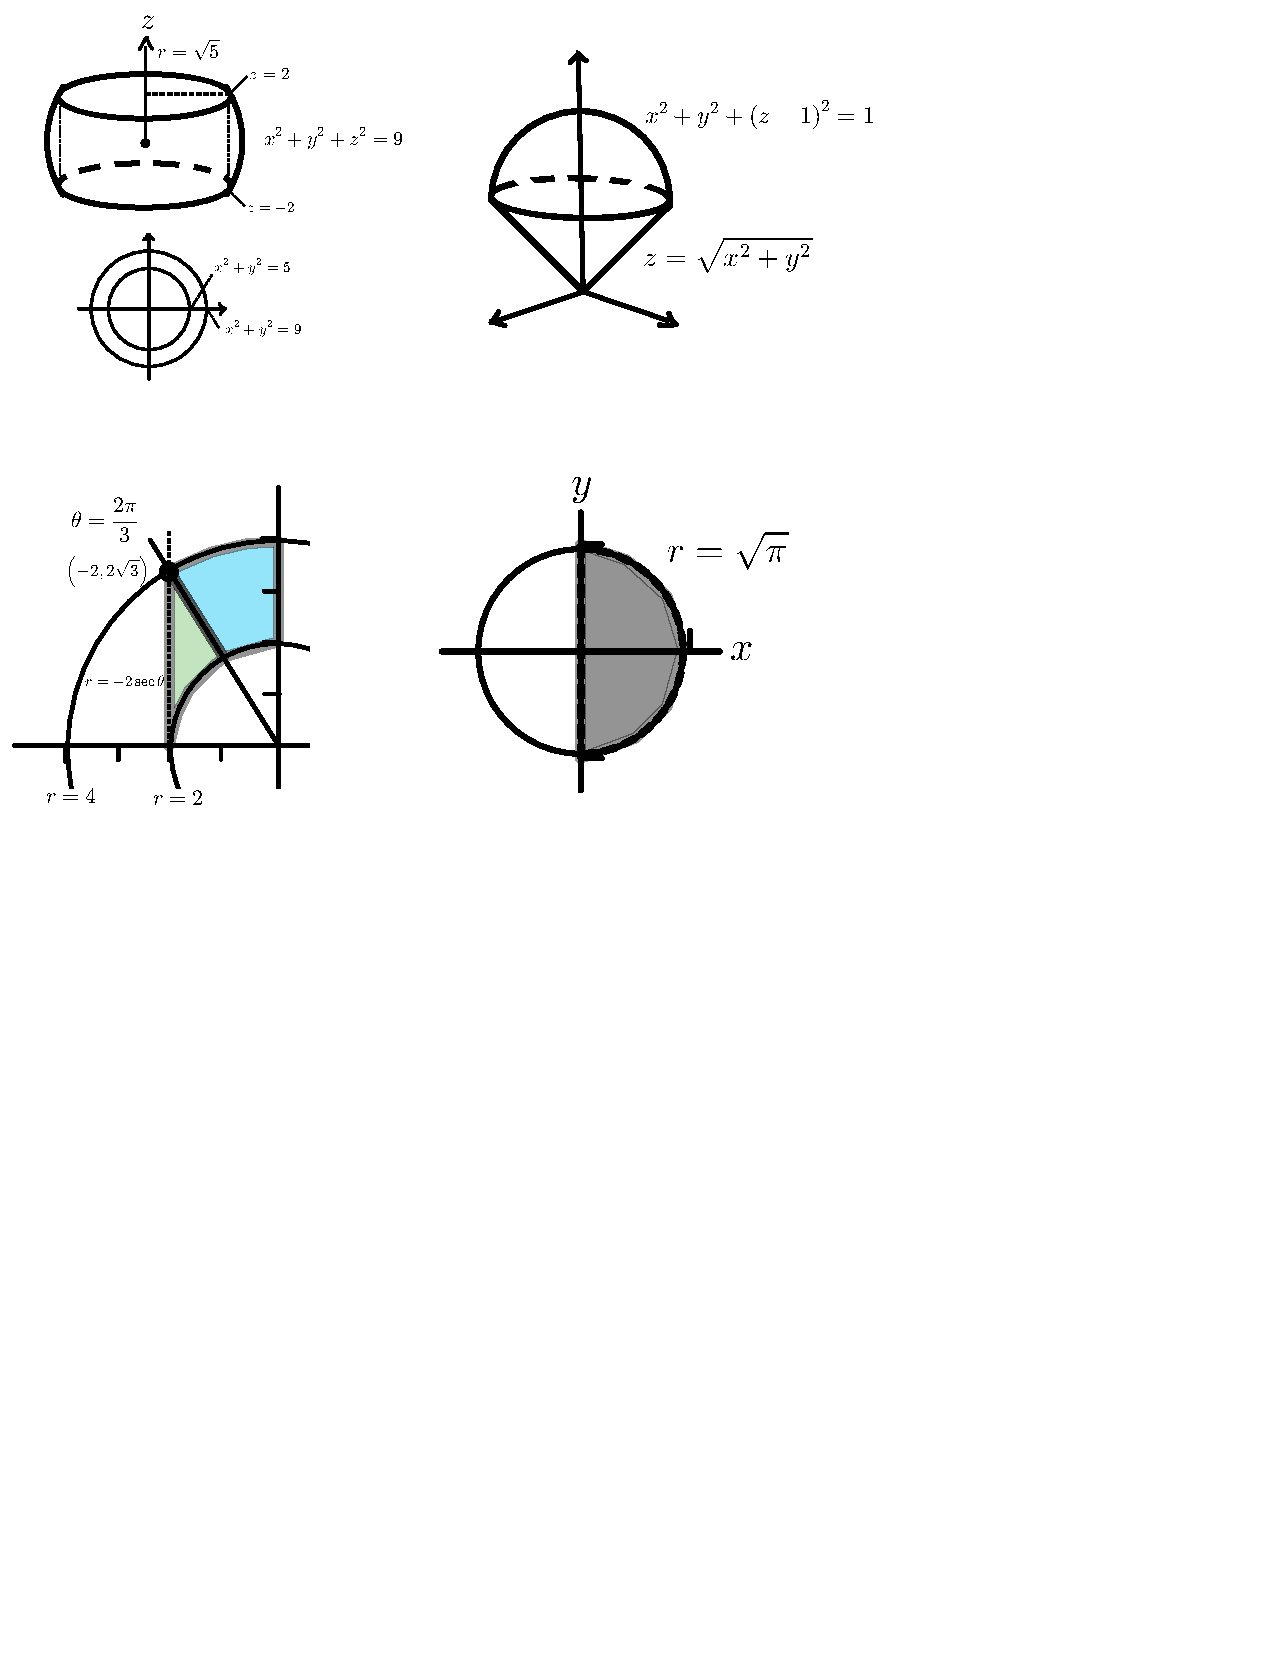
\includegraphics[width=0.5\textwidth, trim=0.7cm 22cm 14.7cm 0.5cm,clip]{figs.pdf} 
\end{flushleft}
\begin{flushright}
\framebox(300,50){}
\end{flushright}

\item Now you're holding an \textbf{ice cream cone}, and you want to find its volume. The solid is enclosed by
$$z=\sqrt{x^2+y^2}, \quad \text{and} \quad x^2+y^2+(z-1)^2=1.$$
Using cylindrical coordinates, set up an integral that computes the volume of this solid.
\begin{flushleft}
    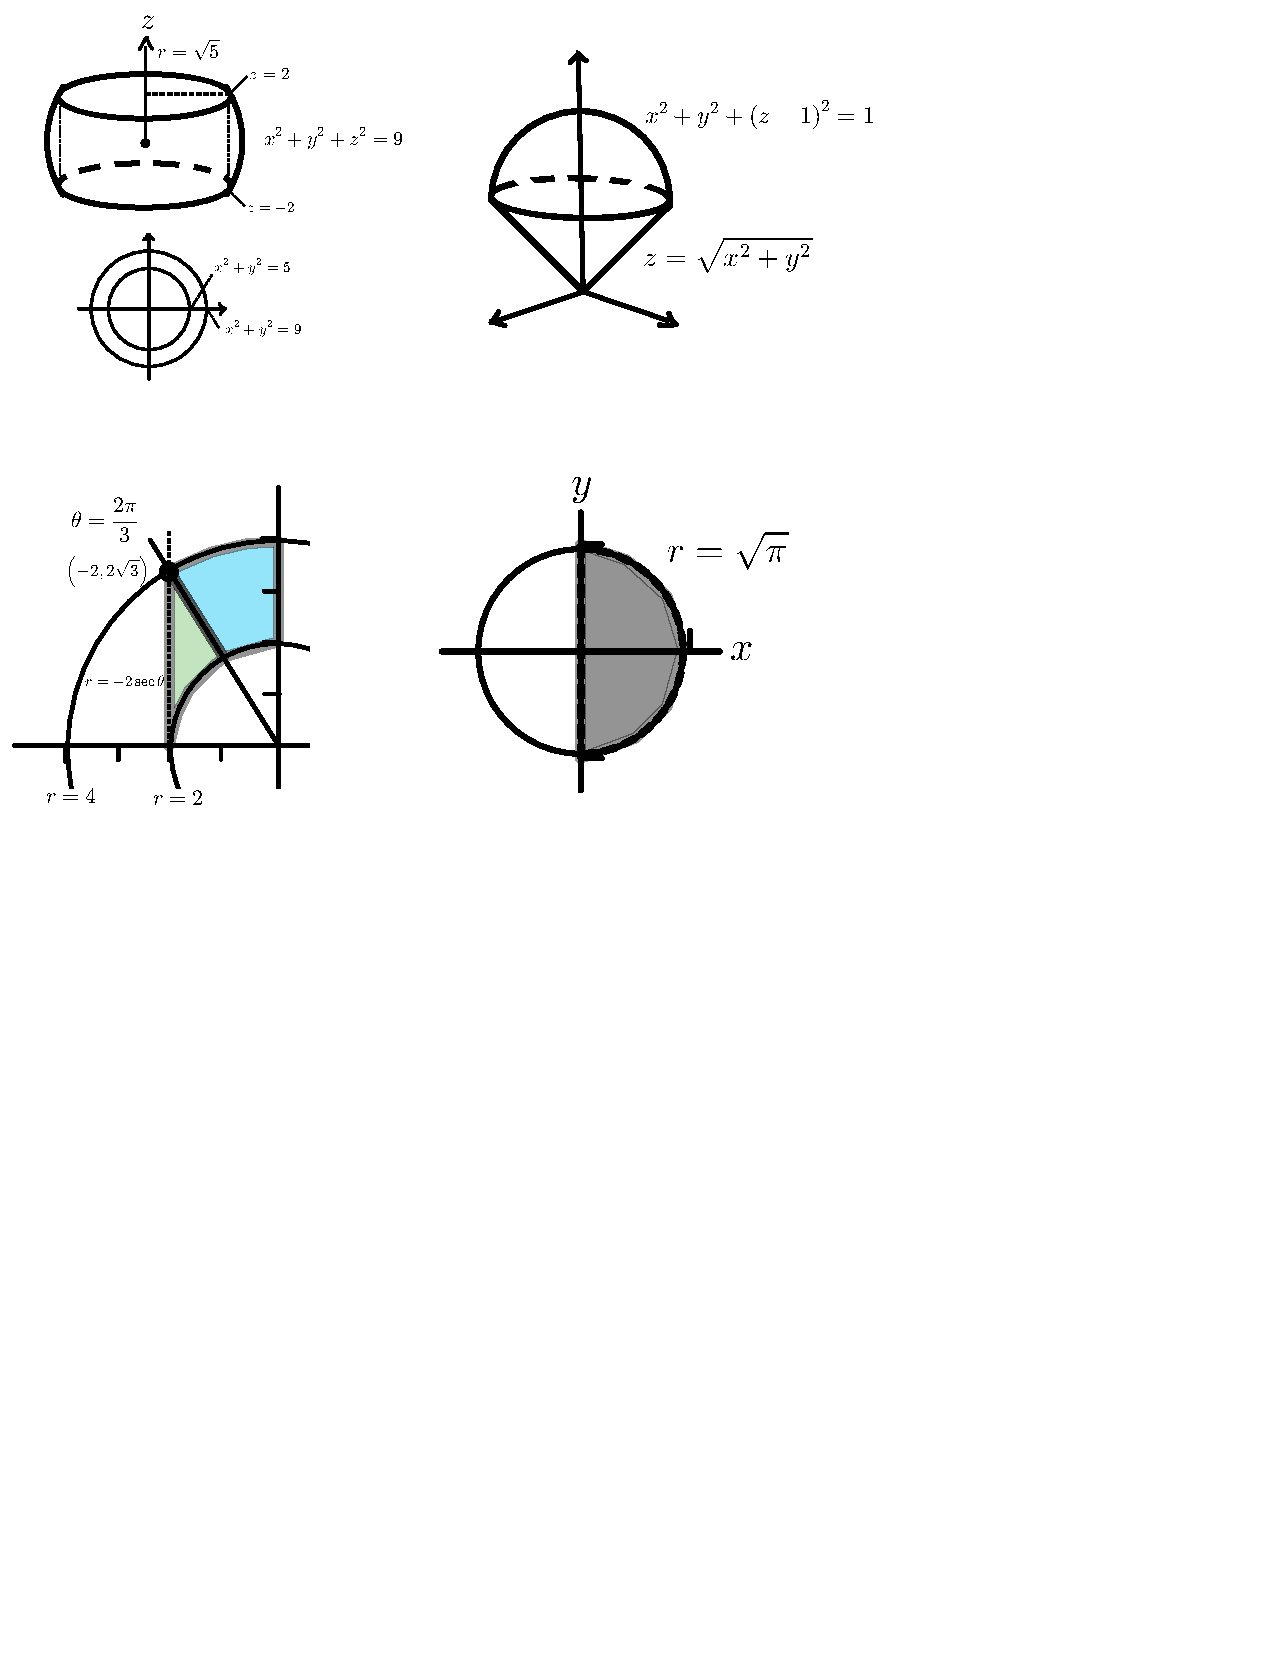
\includegraphics[width=0.4\textwidth, trim=8cm 22.8cm 6.8cm 0.7cm,clip]{figs.pdf}\hfill
\framebox(280,50){}
\end{flushleft}

\end{enumerate}

\end{document}

